\PassOptionsToPackage{unicode=true}{hyperref} % options for packages loaded elsewhere
\PassOptionsToPackage{hyphens}{url}
%
\documentclass[ignorenonframetext,aspectratio=169]{beamer}
\usepackage{pgfpages}
\setbeamertemplate{caption}[numbered]
\setbeamertemplate{caption label separator}{: }
\setbeamercolor{caption name}{fg=normal text.fg}
\beamertemplatenavigationsymbolsempty
% Prevent slide breaks in the middle of a paragraph:
\widowpenalties 1 10000
\raggedbottom
\setbeamertemplate{part page}{
\centering
\begin{beamercolorbox}[sep=16pt,center]{part title}
  \usebeamerfont{part title}\insertpart\par
\end{beamercolorbox}
}
\setbeamerfont{section title}{size=\Huge}
\setbeamertemplate{section page}{
\centering
\begin{beamercolorbox}[sep=12pt,center]{part title}
  \usebeamerfont{section title}\insertsection\par
\end{beamercolorbox}
}
\setbeamertemplate{subsection page}{
\centering
\begin{beamercolorbox}[sep=8pt,center]{part title}
  \usebeamerfont{subsection title}\insertsubsection\par
\end{beamercolorbox}
}
\AtBeginPart{
  \frame{\partpage}
}
\AtBeginSection{
  \ifbibliography
  \else
    \frame{\sectionpage}
  \fi
}
\AtBeginSubsection{
  \frame{\subsectionpage}
}
\usepackage{lmodern}
\usepackage{amssymb,amsmath}
\usepackage{ifxetex,ifluatex}
\usepackage{fixltx2e} % provides \textsubscript
\ifnum 0\ifxetex 1\fi\ifluatex 1\fi=0 % if pdftex
  \usepackage[T1]{fontenc}
  \usepackage[utf8]{inputenc}
  \DeclareUnicodeCharacter{03B5}{$\epsilon$}
  \DeclareUnicodeCharacter{03C3}{$\sigma$}
  \DeclareUnicodeCharacter{03BC}{$\mu$}
  \usepackage{textcomp} % provides euro and other symbols
\else % if luatex or xelatex
  \usepackage{unicode-math}
  \defaultfontfeatures{Ligatures=TeX,Scale=MatchLowercase}
\fi
% use upquote if available, for straight quotes in verbatim environments
\IfFileExists{upquote.sty}{\usepackage{upquote}}{}
% use microtype if available
\IfFileExists{microtype.sty}{%
\usepackage[]{microtype}
\UseMicrotypeSet[protrusion]{basicmath} % disable protrusion for tt fonts
}{}
\IfFileExists{parskip.sty}{%
\usepackage{parskip}
}{% else
\setlength{\parindent}{0pt}
\setlength{\parskip}{6pt plus 2pt minus 1pt}
}
\usepackage{hyperref}
\hypersetup{
            pdfborder={0 0 0},
            breaklinks=true}
\urlstyle{same}  % don't use monospace font for urls
\newif\ifbibliography
\usepackage{color}
\usepackage{fancyvrb}
\newcommand{\VerbBar}{|}
\newcommand{\VERB}{\Verb[commandchars=\\\{\}]}
\DefineVerbatimEnvironment{Highlighting}{Verbatim}{commandchars=\\\{\}}
% Add ',fontsize=\small' for more characters per line
\newenvironment{Shaded}{}{}
\newcommand{\AlertTok}[1]{\textcolor[rgb]{1.00,0.00,0.00}{\textbf{#1}}}
\newcommand{\AnnotationTok}[1]{\textcolor[rgb]{0.38,0.63,0.69}{\textbf{\textit{#1}}}}
\newcommand{\AttributeTok}[1]{\textcolor[rgb]{0.49,0.56,0.16}{#1}}
\newcommand{\BaseNTok}[1]{\textcolor[rgb]{0.25,0.63,0.44}{#1}}
\newcommand{\BuiltInTok}[1]{#1}
\newcommand{\CharTok}[1]{\textcolor[rgb]{0.25,0.44,0.63}{#1}}
\newcommand{\CommentTok}[1]{\textcolor[rgb]{0.38,0.63,0.69}{\textit{#1}}}
\newcommand{\CommentVarTok}[1]{\textcolor[rgb]{0.38,0.63,0.69}{\textbf{\textit{#1}}}}
\newcommand{\ConstantTok}[1]{\textcolor[rgb]{0.53,0.00,0.00}{#1}}
\newcommand{\ControlFlowTok}[1]{\textcolor[rgb]{0.00,0.44,0.13}{\textbf{#1}}}
\newcommand{\DataTypeTok}[1]{\textcolor[rgb]{0.56,0.13,0.00}{#1}}
\newcommand{\DecValTok}[1]{\textcolor[rgb]{0.25,0.63,0.44}{#1}}
\newcommand{\DocumentationTok}[1]{\textcolor[rgb]{0.73,0.13,0.13}{\textit{#1}}}
\newcommand{\ErrorTok}[1]{\textcolor[rgb]{1.00,0.00,0.00}{\textbf{#1}}}
\newcommand{\ExtensionTok}[1]{#1}
\newcommand{\FloatTok}[1]{\textcolor[rgb]{0.25,0.63,0.44}{#1}}
\newcommand{\FunctionTok}[1]{\textcolor[rgb]{0.02,0.16,0.49}{#1}}
\newcommand{\ImportTok}[1]{#1}
\newcommand{\InformationTok}[1]{\textcolor[rgb]{0.38,0.63,0.69}{\textbf{\textit{#1}}}}
\newcommand{\KeywordTok}[1]{\textcolor[rgb]{0.00,0.44,0.13}{\textbf{#1}}}
\newcommand{\NormalTok}[1]{#1}
\newcommand{\OperatorTok}[1]{\textcolor[rgb]{0.40,0.40,0.40}{#1}}
\newcommand{\OtherTok}[1]{\textcolor[rgb]{0.00,0.44,0.13}{#1}}
\newcommand{\PreprocessorTok}[1]{\textcolor[rgb]{0.74,0.48,0.00}{#1}}
\newcommand{\RegionMarkerTok}[1]{#1}
\newcommand{\SpecialCharTok}[1]{\textcolor[rgb]{0.25,0.44,0.63}{#1}}
\newcommand{\SpecialStringTok}[1]{\textcolor[rgb]{0.73,0.40,0.53}{#1}}
\newcommand{\StringTok}[1]{\textcolor[rgb]{0.25,0.44,0.63}{#1}}
\newcommand{\VariableTok}[1]{\textcolor[rgb]{0.10,0.09,0.49}{#1}}
\newcommand{\VerbatimStringTok}[1]{\textcolor[rgb]{0.25,0.44,0.63}{#1}}
\newcommand{\WarningTok}[1]{\textcolor[rgb]{0.38,0.63,0.69}{\textbf{\textit{#1}}}}
\usepackage{graphicx,grffile}
\makeatletter
\def\maxwidth{\ifdim\Gin@nat@width>\linewidth\linewidth\else\Gin@nat@width\fi}
\def\maxheight{\ifdim\Gin@nat@height>\textheight\textheight\else\Gin@nat@height\fi}
\makeatother
% Scale images if necessary, so that they will not overflow the page
% margins by default, and it is still possible to overwrite the defaults
% using explicit options in \includegraphics[width, height, ...]{}
\setkeys{Gin}{width=\maxwidth,height=\maxheight,keepaspectratio}
\setlength{\emergencystretch}{3em}  % prevent overfull lines
\providecommand{\tightlist}{%
  \setlength{\itemsep}{0pt}\setlength{\parskip}{0pt}}
\setcounter{secnumdepth}{0}

% set default figure placement to htbp
\makeatletter
\def\fps@figure{htbp}
\makeatother



\begin{document}


\begin{frame}
\color{blue}
\begin{center}
    \begin{Huge}
        MD-Bench
    \end{Huge}

\begin{huge}
    GPU port optimization
\end{huge}

\color{black}

by: Martin Bauernfeind

advised by: Rafael Ravedutti
\end{center}

\end{frame}

\section{Project Description}


\begin{frame}{Project description}{Application Info}
    \begin{itemize}
        \item original MD-Bench:
        \begin{itemize}
            \item mini-app to simulate molecular dynamics
            \item written in sequential C with less than 1000 lines of code
        \end{itemize}
        \vspace{\baselineskip}
        \item MD-Bench on Cuda:
        \begin{itemize}
            \item port MD-Bench to Cuda to use GPGPU parallelism
            \item significant parts not ported yet
        \end{itemize}
        \vspace{\baselineskip}
        \tightlist
        \item
        Code: MD-Bench on Cuda
        \item
        URL:
        \href{https://github.com/RRZE-HPC/MD-Bench/tree/mucosim_cuda}{https://github.com/RRZE-HPC/MD-Bench/tree/mucosim\_cuda}
    \end{itemize}
\end{frame}

\begin{frame}{Project Description}{Simulation Model}
    Molecular dynamics emulated in MD-Bench by:
    \begin{itemize}
        \vspace*{-0.5\baselineskip}
        \tightlist
        \item interaction among particles
        \item affects of these interactions on their motion
        \item constituents of simulation:
        \begin{itemize}
            \item Number of atoms with initial state (position \& velocity)
            \item Boundary conditions (periodic)
        \end{itemize}
    \end{itemize}
    \begin{center}
        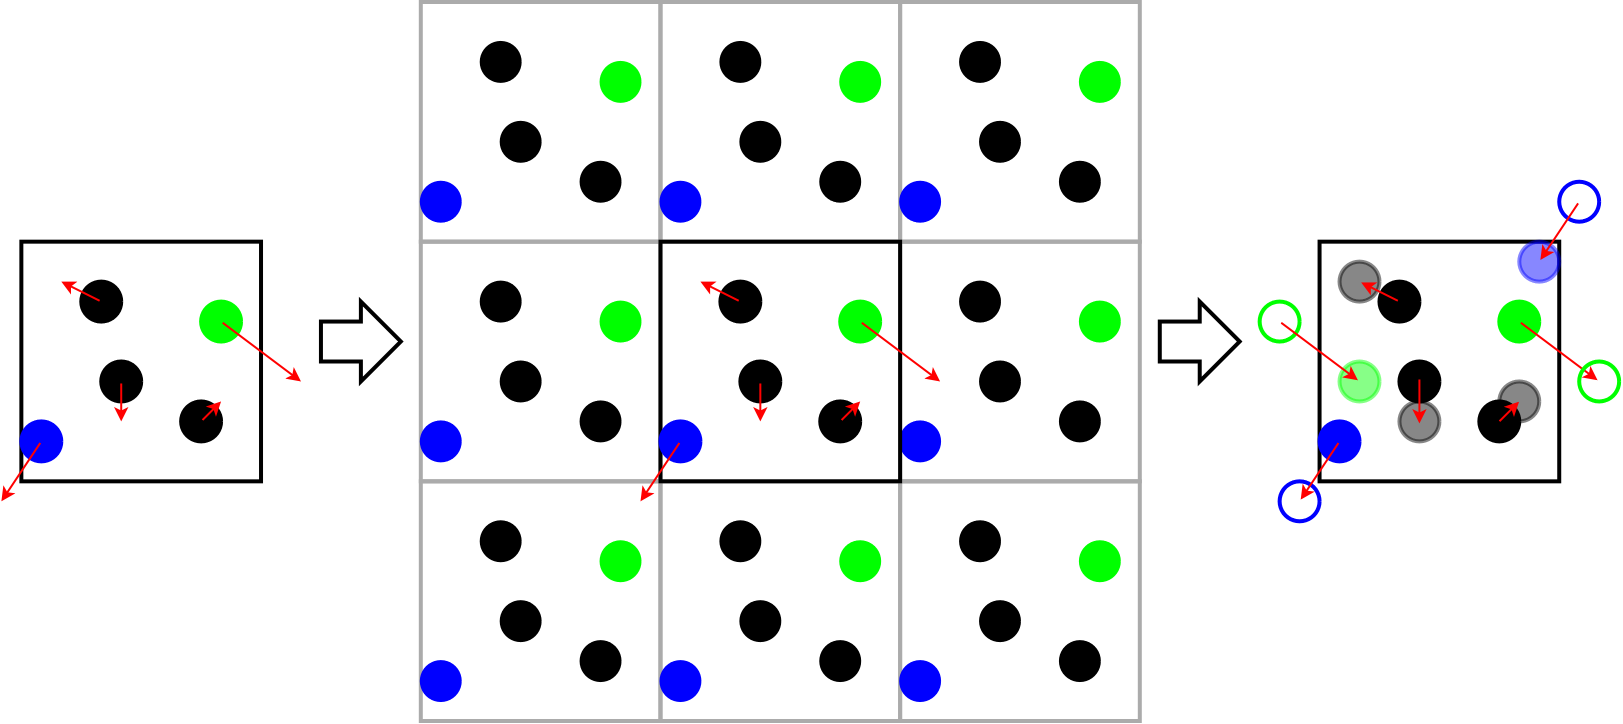
\includegraphics[width=0.6\linewidth]{../images/Boundary_Condition_explained_without_ghosts.png}
    \end{center}
\end{frame}

\begin{frame}{Project Description}{Particle interactions} 
    force computation of particle interactions:
    \begin{itemize}
        \tightlist
        \vspace*{-0.3\baselineskip}
        \item
          based on the Lennard-Jones potential:
          \begin{itemize}

              \tightlist
              \item pairs of particles, here: electronically neutral atoms
              \item models repulsive as well as attractive interactions
          \end{itemize}
    \end{itemize}
    \begin{center}
        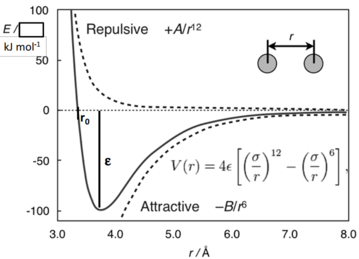
\includegraphics[width=0.35\textwidth]{../images/Lennard_Jones_potential_function.png}
    \end{center}
    
    
    \begin{itemize}
        \tightlist
        \item
          \emph{\textbf{r}} is the distance between the two interacting atoms,
        \item
          \emph{\textbf{ε}} is the dispersion energy and
        \item
          \emph{\textbf{σ}} the distance at which the particle-potential
          \emph{\textbf{V}} is zero
    \end{itemize}
\end{frame}

\begin{frame}[fragile]{Project Description}{Simulation Process}
    
    The simulation runs similar to the sketch code below:
    
    \begin{itemize}
        \tightlist
        \item every timestep iterate over all particles:
          \begin{itemize}
              \tightlist
              \item compute interactions with neighbors
              \item integrate force generated by interaction
          \end{itemize}
    \end{itemize}
    
    \begin{scriptsize}
    \begin{Shaded}
    \begin{Highlighting}[]
    \ControlFlowTok{for}\NormalTok{ t }\KeywordTok{in}\NormalTok{ timesteps:}
      \ControlFlowTok{for}\NormalTok{ atom }\KeywordTok{in}\NormalTok{ atoms:}
    \NormalTok{    velocity[atom] }\OperatorTok{+=}\NormalTok{ force[atom]}
    \NormalTok{    position[atom] }\OperatorTok{+=}\NormalTok{ velocity[atom]}
      \ControlFlowTok{if}\NormalTok{ t }\OperatorTok{%} \DecValTok{20} \OperatorTok{==} \DecValTok{0}\NormalTok{:}
    \NormalTok{    neighbors }\OperatorTok{=}\NormalTok{ calculateNeighbors()}
      \ControlFlowTok{for}\NormalTok{ atom }\KeywordTok{in}\NormalTok{ atoms:}
    \NormalTok{    neighbors }\OperatorTok{=}\NormalTok{ neighbors[atom]}
    \NormalTok{    force }\OperatorTok{=} \FloatTok{0.0}
        \ControlFlowTok{for}\NormalTok{ neighbor }\KeywordTok{in}\NormalTok{ neighbors:}
    \NormalTok{        radius }\OperatorTok{=}\NormalTok{ calc_radius(...)}
            \ControlFlowTok{if}\NormalTok{ radius }\OperatorTok{<}\NormalTok{ close_enough:}
    \NormalTok{            force }\OperatorTok{+=}\NormalTok{ calc_force(...)}
    \NormalTok{    forces[atom] }\OperatorTok{+=}\NormalTok{ force}
    \end{Highlighting}
    \end{Shaded}
    \end{scriptsize}
\end{frame}

\section{Testsystem}

\begin{frame}{Testsystem}    
    \begin{itemize}
        \tightlist
        \item Host/Clustername: alex
        \item multiple nodes with multiple GPUs per node
        \item
          resources per GPU:
        
          \begin{itemize}
          \tightlist
          \item
            {[}A40 \textbar{} A100{]}
          \item
            CPU: {[}16 cores / GPU \textbar{} 16 cores / GPU{]}
          \item
            Memory: {[}60GB / GPU \textbar{} 120GB / GPU{]}
          \end{itemize}
        \item computational power
        \begin{itemize}
            \item SP: {[}A40: 37.4 TFlops \textbar{} A100: 19.5 Tflops {]}
            \item DP: {[}A40: 0.5 TFlops \textbar{} A100: 9.7 Tflops {]}
        \end{itemize}
    \end{itemize}
    
    \textbf{Note}: each an A40 has about double the single precision
    processing power of an A100 despite being cheaper
\end{frame}

\section{Execution and default parameters}

\begin{frame}[fragile]{Executing the simulation}
    \begin{block}{Software Environment}
        \begin{itemize}
            \tightlist
            \item Compiler: NVCC (cuda/11.6.1)
            \item Operating System: Ubuntu 20.04.3 LTS
            \item Addition libraries:
            \begin{itemize}
                \tightlist
                \item LIKWID 5.2.0
            \end{itemize}
        \end{itemize}
    \end{block}
    
    \begin{block}{How to build software}
        \begin{verbatim}
$ git clone https://github.com/RRZE-HPC/MD-Bench/
$ cd MD-Bench
$ git checkout mucosim_cuda
$ module load likwid cuda
$ make
        \end{verbatim}
    \end{block}
    \vspace{-\baselineskip}
    \begin{block}{How to run software (e.g. in a batch job)}
        \begin{verbatim}
$ module load likwid cuda
$ cd MD-Bench
$ ./MDBench-NVCC
        \end{verbatim}
    \end{block}
\end{frame}

\begin{frame}[fragile]{Testcase description}
    \vspace*{-6\baselineskip}
    If not stated otherwise these are the conditions for the simulation benchmarking.
    
    \begin{itemize}
        \tightlist
        \item the number of simulated atoms is 131072
        \item floating point numbers use double precision
        \item force computation between atoms uses the lennard-jones model
        \item one gpu with its associated cores are used for computation
    \end{itemize}

\end{frame}



\begin{frame}[fragile]{First runtime tests}{Scaling GPU-Threads per thread block}
    \begin{itemize}
        \item plot data for single- and double precision performance
    \end{itemize}
    \begin{center}
        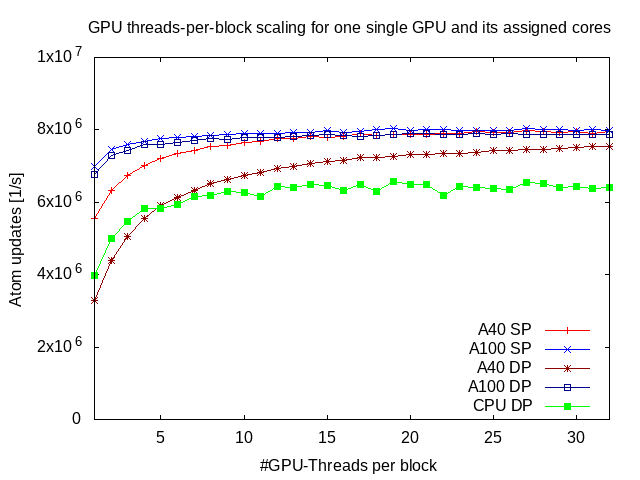
\includegraphics[width=0.5\linewidth]{../resources/initial_testing/linear_cpu-threads_scaling/SingleGPU_gpu_threads_per_block_scaling.png}
    \end{center}

Similar convergence points in performance between the A40 and A100 hints at bottlenecks independent of the gpu.

\end{frame}

\section{Profiling the application}

\begin{frame}[fragile]{Profiling the application}{Using nsys}

		\begin{verbatim}
    srun nsys profile -o ./a40_profiling_run
		\end{verbatim}
    \begin{itemize}
    	\item to get this runtime timeline:
    \end{itemize}

    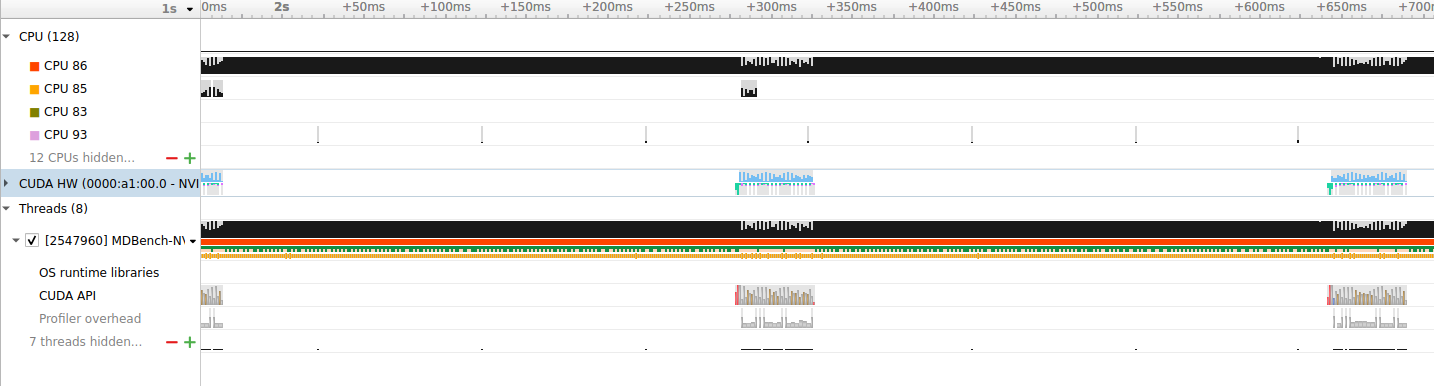
\includegraphics{../resources/initial_testing/finding_bottlenecks/using_nsys/A40_nsys_zoomed_in.png}

    \begin{itemize}
        \tightlist
        \item activity is cyclic
        \item most of the time is spent with only one CPU active
        \item short blue parts are where the GPU is active
    \end{itemize}
\end{frame}

\begin{frame}[fragile]{Profiling the application}{Finding where the CPU time is spent}
    \begin{itemize}
    	\item using \texttt{gprof}
    	\begin{itemize}
    		\item GPU time is not counted as such here
    	\end{itemize}
    \end{itemize}

    \begin{verbatim}
Flat profile:
Each sample counts as 0.01 seconds.
  %      self              total           
 time   seconds    calls  ms/call  name    
 97.70     3.35       11   306.47  buildNeighbor
  0.87     0.03      201     0.15  updatePbc
  0.58     0.02  2359296     0.00  myrandom
  0.58     0.02       11     1.82  binatoms
  0.29     0.01       11     0.91  setupPbc
  0.00     0.00     1668     0.00  checkCUDAError
  0.00     0.00      426     0.00  getTimeStamp
  0.00     0.00      201     0.00  computeForce
...
    \end{verbatim}
\end{frame}

\begin{frame}[fragile]{Profiling the application}{using runtime readings inside the program}
\vspace{-4\baselineskip}
    \begin{itemize}
    	\item in the standard program output
    	\begin{itemize}
    		\item tracks total time
    		\item takes both CPU and GPU into account
    		\item total runtime spent on the different phases
    	\end{itemize}
    \end{itemize}
    
    Even when considering CPU and GPU time the neighbor calculation needs most of the time.
\end{frame}




\begin{frame}{Next goals}
    \vspace{-3\baselineskip}
    \begin{itemize}
        \item port the buildNeighbor-function to Cuda
    \begin{itemize}
        \item reduces Host-To-Device traffic
        \item reduces computation time
    \end{itemize}
    \item port function updating the ghost atoms to Cuda
    \item port creating the ghost atoms to Cuda
    
    \vspace{\baselineskip}
    \item evaluate performance along the way
    \end{itemize}


\end{frame}

\section{Parallelizing building neighbor lists}

\begin{frame}{Effects on runtime}{Parallelizing building neighbor lists}
    
    
    program output on runtimes of different parts
    \begin{itemize}
        \tightlist
        \item
        A40:
        
        \begin{itemize}
            \tightlist
            \item
            Before:~\texttt{TOTAL\ 3.46s\ FORCE\ 0.21s\ NEIGH\ 3.14s\ REST\ 0.12s}
            \item
            After:~~~\texttt{TOTAL\ 0.37s\ FORCE\ 0.21s\ NEIGH\ 0.06s\ REST\ 0.09s}
        \end{itemize}
        \item
        A100:
        
        \begin{itemize}
            \tightlist
            \item
            Before:~\texttt{TOTAL\ 3.01s\ FORCE\ 0.05s\ NEIGH\ 2.84s\ REST\ 0.12s}
            \item
            After:~~~\texttt{TOTAL\ 0.18s\ FORCE\ 0.05s\ NEIGH\ 0.04s\ REST\ 0.10s}
        \end{itemize}
    \end{itemize}
\end{frame}
\begin{frame}{Effects on runtime profile}{Parallelizing building neighbor lists}
    \begin{center}
        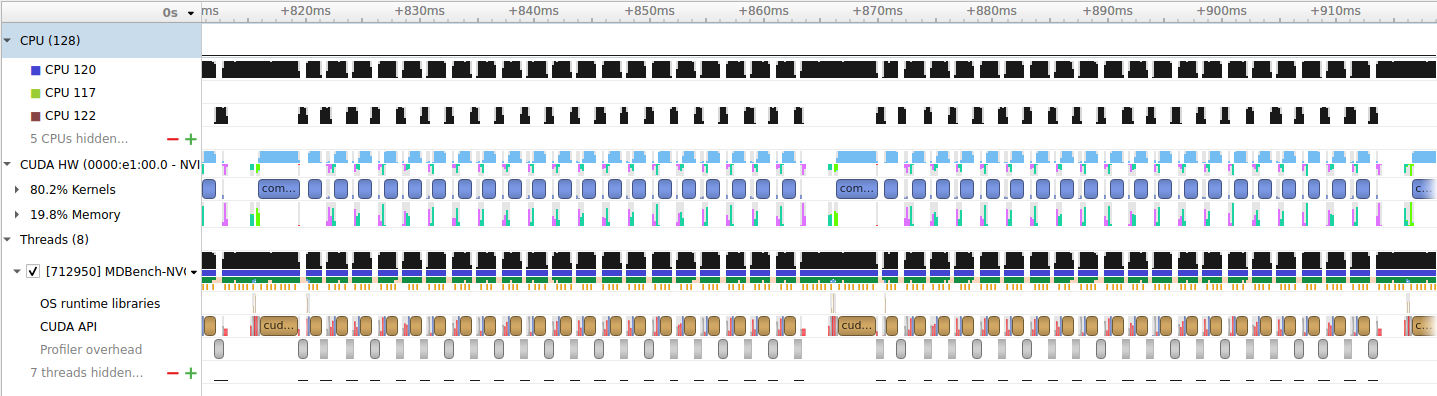
\includegraphics{../resources/profiling/nsys/a40_buiNei_profile.png}
    \end{center}
\end{frame}

\begin{frame}{Effects on performance}{Parallelizing building neighbor lists}
    \begin{itemize}
        \tightlist
        \item
        A40:
        
        \begin{itemize}
            \tightlist
            \item
            Before:~\texttt{Performance:\ 7.59\ million\ atom\ updates\ per\ second}
            \item
            After:~~~\texttt{Performance:\ 71.79\ million\ atom\ updates\ per\ second}
        \end{itemize}
        \item
        A100
        
        \begin{itemize}
            \tightlist
            \item
            Before:~\texttt{Performance:\ 7.93\ million\ atom\ updates\ per\ second}
            \item
            After:~~~\texttt{Performance:\ 143.60\ million\ atom\ updates\ per\ second}
        \end{itemize}
    \end{itemize}

    
    
    

\end{frame}

\begin{frame}[fragile]{Effects on memory traffic}{Parallelizing building neighbor lists}
    
    \begin{itemize}
        \item from:
    \end{itemize}
    \begin{verbatim}
    Total       Count   Min         Max         Operation
    1,36 GiB    229     128 B       50,00 MiB   [CUDA memcpy HtoD]
    660,00 MiB  220     3,00 MiB    3,00 MiB    [CUDA memcpy DtoH]
    \end{verbatim}

    \begin{itemize}
    \item to:
    \end{itemize}    
    
    
    \begin{verbatim}
    Total       Count   Min         Max         Operation
    881,28 MiB  240     128 B       4,12 MiB    [CUDA memcpy HtoD]
    660,00 MiB  231     4 B         3,00 MiB    [CUDA memcpy DtoH]
    44 B        11      4 B         4 B         [CUDA memset]
    \end{verbatim}
    
\end{frame}

\begin{frame}[fragile]{Effects on scaling}{Parallelizing building neighbor lists}
    \begin{columns}[T] % align columns
        \begin{column}{.36\linewidth}
            \begin{itemize}
                \item BL - baseline \newline 
                (only force GPU-parallel) \newline
                $\Downarrow$ port neighbor list constr.
                \item NL
            \end{itemize}

            
        \end{column}%
        \hfill%
        \begin{column}{.7\linewidth}
            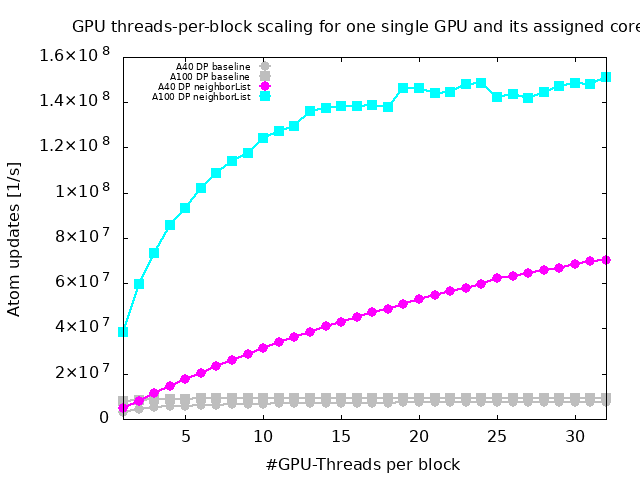
\includegraphics[width=\linewidth]{../resources/development_stage_comparisons/t200_DP_scaling_comparisons/plot_upto_buiNeiPar.png}
        \end{column}%
    \end{columns}
\end{frame}


\section{Parallelizing further components}
\begin{frame}{Parallelizing updatePbc}{Parallelizing further components}
    \begin{columns}[T] % align columns
    \begin{column}{.36\linewidth}
        \begin{itemize}
            \item BL: baseline \newline 
            (only force GPU-parallel) \newline
            $\Downarrow$ port neighbor list constr.
            \item NL \newline
            $\Downarrow$ port updatePbc
            \item UP \newline
        \end{itemize}
        
        
    \end{column}%
    \hfill%
    \begin{column}{.7\linewidth}
        \includegraphics[width=\linewidth]{../resources/development_stage_comparisons/t200_DP_scaling_comparisons/plot_upto_PbcPar.png}
    \end{column}%
    \end{columns}
\end{frame}

\begin{frame}{Parallelizing binAtoms}{Parallelizing further components}
    \begin{columns}[T] % align columns
    \begin{column}{.36\linewidth}
        \begin{itemize}
            \item BL: baseline \newline 
            (only force GPU-parallel) \newline
            $\Downarrow$ port neighbor list constr.
            \item NL \newline
            $\Downarrow$ port updatePbc
            \item UP \newline
            $\Downarrow$ port binAtoms
            \item BA \newline
        \end{itemize}
        
        
    \end{column}%
    \hfill%
    \begin{column}{.7\linewidth}
        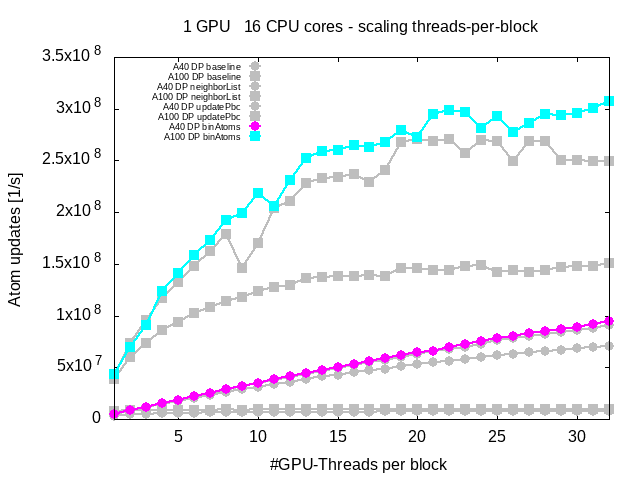
\includegraphics[width=\linewidth]{../resources/development_stage_comparisons/t200_DP_scaling_comparisons/plot_upto_binAtPar.png}
    \end{column}%
\end{columns}
\end{frame}

\begin{frame}{Parallelizing updateAtomsPbc}{Parallelizing further components}
    \begin{columns}[T] % align columns
    \begin{column}{.36\linewidth}
        \begin{itemize}
            \item BL: baseline \newline 
            (only force GPU-parallel) \newline
            $\Downarrow$ port neighbor list constr.
            \item NL \newline
            $\Downarrow$ port updatePbc
            \item UP \newline
            $\Downarrow$ port binAtoms
            \item BA \newline
            $\Downarrow$ port updateAtomsPbc
            \item UAP
        \end{itemize}
        
        
    \end{column}%
    \hfill%
    \begin{column}{.7\linewidth}
        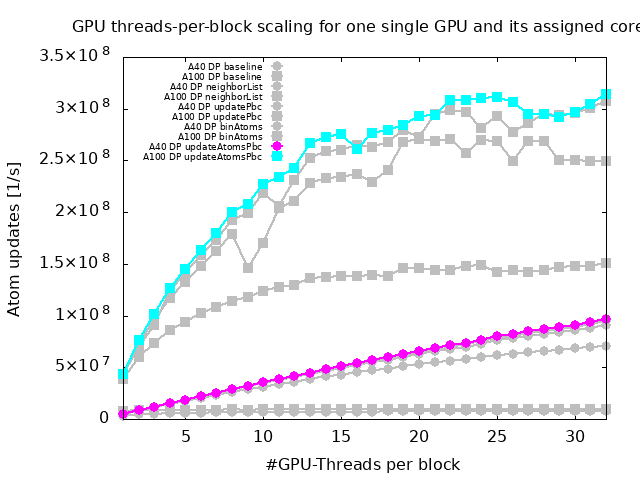
\includegraphics[width=\linewidth]{../resources/development_stage_comparisons/t200_DP_scaling_comparisons/plot_upto_upAtPar.png}
    \end{column}%
\end{columns}
\end{frame}

\begin{frame}[fragile]{Very low runtimes after parallelization}{Parallelizing further components}
    
    \begin{itemize}
        \tightlist
        \item
        A40:
    \end{itemize}
    
    \begin{verbatim}
    TOTAL 0.27s FORCE 0.21s NEIGH 0.05s REST 0.01s
    \end{verbatim}
    
    \begin{itemize}
        \tightlist
        \item
        A100:
    \end{itemize}
    
    \begin{verbatim}
    TOTAL 0.09s FORCE 0.05s NEIGH 0.03s REST 0.01s
    \end{verbatim}

\begin{itemize}
    \item high variations in throughput caused by small variations in runtime
    \begin{itemize}
        \item increase workload
    \end{itemize}
\end{itemize}    
\end{frame}

\section{Measurements after parallelization}

\begin{frame}[fragile]{Increasing workload}{Measurements after parallelization}
    \begin{itemize}
        \item increase workload
        \begin{itemize}
            \item timesteps: 200 $\rightarrow$ 2000
            \item atoms in domain: 128Ki $\rightarrow$ 1Mi
        \end{itemize}
    \end{itemize}


\begin{itemize}
    \tightlist
    \item
    A40:\begin{verbatim}
    System: 1048576 atoms 173434 ghost atoms, Steps: 2000
    TOTAL 19.57s FORCE 15.49s NEIGH 3.15s REST 0.93s
    \end{verbatim}
\end{itemize}



\begin{itemize}
    \tightlist
    \item
    A100:\begin{verbatim}
    System: 1048576 atoms 173434 ghost atoms, Steps: 2000
    TOTAL 4.27s FORCE 2.14s NEIGH 1.54s REST 0.59s
    \end{verbatim}
\end{itemize}

\end{frame}

\begin{frame}{Looking at the runtime profile}{Measurements after parallelization}
    \begin{itemize}
        \item gaps in the runtime are due to the profiler flushing its buffers
    \end{itemize}
    \begin{center}
        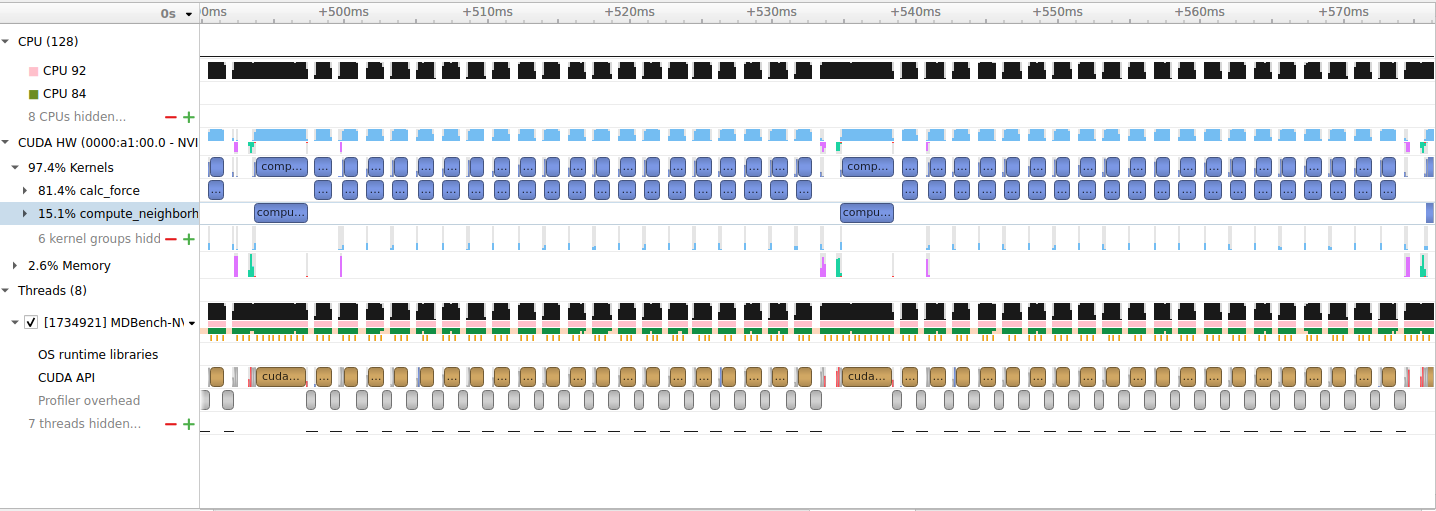
\includegraphics{../resources/profiling/nsys/a40_upAt_profile.png}
    \end{center}
\end{frame}

\begin{frame}[fragile]{Looking at the runtime profile - continued}{Measurements after parallelization}
    \begin{itemize}
        \item memory still takes quite some time
    \end{itemize}
\begin{verbatim}
Time Total Time        Count   Min       Max         Operation
67.0%      310,648 ms  523     1,344 μs  475,849 μs  [CUDA memcpy DtoH]
32.0%      150,418 ms  613     1,023 μs  411,571 μs  [CUDA memcpy HtoD]
0.0%       519,530 μs  307     991 ns    898 ns      [CUDA memset]
\end{verbatim}

\begin{itemize}
    \item $\sum$ $\approx$ 460 ms = 0.46s
    \item recall:
    \begin{itemize}
        \item A40 runtime: ~19.5s
        \item A100 runtime: ~4.3s
    \end{itemize}
\end{itemize}
\end{frame}

\begin{frame}[fragile]{Runtime spent in the neighbor computation}{Measurements after parallelization}
    \begin{itemize}
        \item A40\begin{verbatim}
        NEIGH 3.15s
        NEIGH_TIMERS: 
        UPDATE_ATOMS: 0.10s         SETUP_PBC 0.57s 
        UPDATE_PBC    0.20s         BINATOMS 0.02s 
        BUILD_NEIGHBOR 2.31s
        \end{verbatim}
        \item A100 \begin{verbatim}
        NEIGH 1.54s 
        NEIGH_TIMERS: 
        UPDATE_ATOMS: 0.11s         SETUP_PBC 0.49s 
        UPDATE_PBC    0.19s         BINATOMS 0.02s 
        BUILD_NEIGHBOR 0.78s
        \end{verbatim}
    \end{itemize}
\end{frame}

\section{Finding peak performance}

\begin{frame}{Scaling beyond 32 blocks per thread - A40}{Finding peak performance}
    \begin{center}
        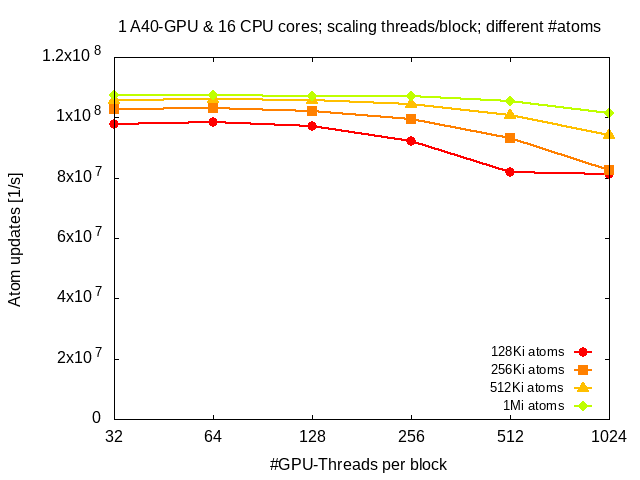
\includegraphics[width=0.7\linewidth]{../resources/scaling/exponential_thread_scaling/gpu32-1024_t2000_p128K-1M/a40_gpu32-1024_t2000_pScaling.png}
    \end{center}
\end{frame}

\begin{frame}{Scaling beyond 32 blocks per thread - A100}{Finding peak performance}
    \begin{center}
        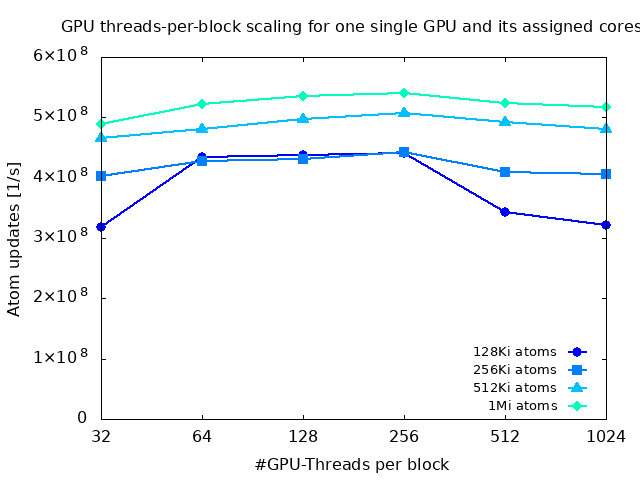
\includegraphics[width=0.7\linewidth]{../resources/scaling/exponential_thread_scaling/gpu32-1024_t2000_p128K-1M/a100_gpu32-1024_t2000_pScaling.png}
    \end{center}
\end{frame}

\begin{frame}{Neighbor List construction performance}{Finding peak performance}
    \begin{center}
        
\includegraphics[width=0.7\linewidth]{../resources/scaling/exponential_thread_scaling/neigh_perf_with_force/buiNeiList_perf.png}
    \end{center}
\end{frame}

\begin{frame}{Force computation performance}{Finding peak performance}
    \begin{center}
        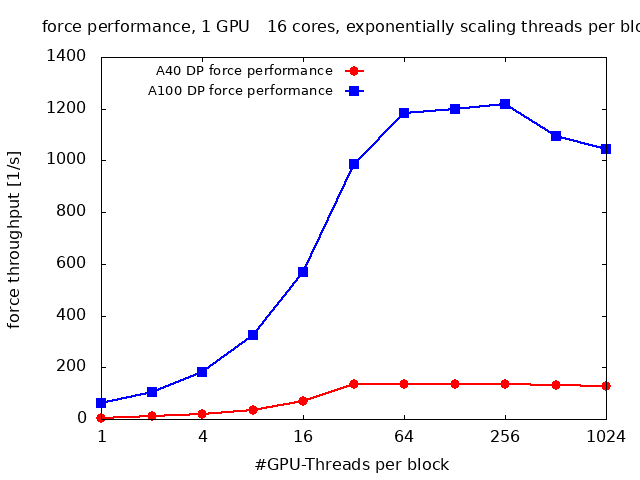
\includegraphics[width=0.7\linewidth]{../resources/scaling/exponential_thread_scaling/neigh_perf_with_force/force_perf.png}
    \end{center}
\end{frame}

\section{Before $\longleftrightarrow$ After \newline Neighborhood calculation porting}

\begin{frame}{Performance comparison}{A40 Before $\longleftrightarrow$ After}
    \begin{columns}
        \begin{column}{0.65\linewidth}
            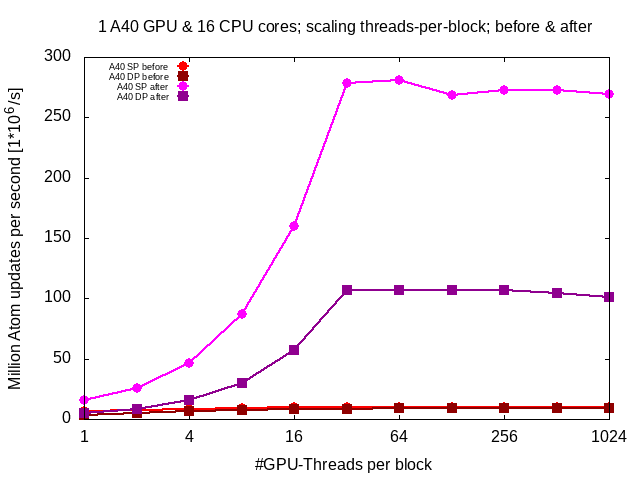
\includegraphics[width=\linewidth]{../resources/before_after_comparison/a40_perf_comp_log_before_after.png}
        \end{column}
        \begin{column}{0.35\linewidth}
        Performance increase:
        \vspace{\baselineskip}
        \begin{itemize}
            \item double precision (DP)
            \begin{itemize}
                \item factor 10 - 11
            \end{itemize}
            \vspace{0.5\baselineskip}
            \item single precision (SP)
            \begin{itemize}
                \item factor 26 - 27
            \end{itemize}
        \end{itemize}
    \end{column}
    \end{columns}
\end{frame}

\begin{frame}{Performance comparison}{A100 Before $\longleftrightarrow$ After}
    \begin{columns}
        \begin{column}{0.65\linewidth}
            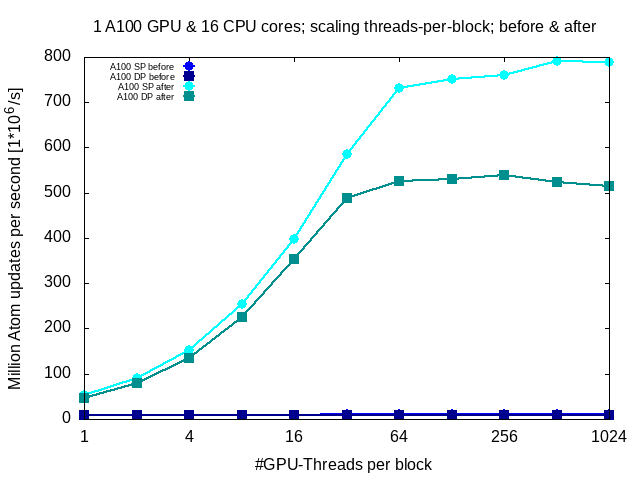
\includegraphics[width=\linewidth]{../resources/before_after_comparison/a100_perf_comp_log_before_after.png}
        \end{column}
        \begin{column}{0.35\linewidth}
            Performance increase:
            \vspace{\baselineskip}
            \begin{itemize}
                \item double precision (DP)
                \begin{itemize}
                    \item factor 55
                \end{itemize}
                \vspace{0.5\baselineskip}
                \item single precision (SP)
                \begin{itemize}
                    \item factor 80
                \end{itemize}
            \end{itemize}
        \end{column}
    \end{columns}
\end{frame}

\section{Outlook}
\begin{frame}{Outlook}
    \begin{itemize}
        \item setupPbc still on CPU
        \begin{itemize}
            \item runtime itself not negligible
            \item requires costly memcpy from device to host and back
            \item difficult to port
        \end{itemize}
        \item kernels mostly still not optimized
    \end{itemize}
\end{frame}

\begin{frame}
    \begin{center}
        \color{blue}
        \begin{Huge}
            Thank you 
            
            for your attention
        \end{Huge}
        \vspace{\baselineskip}
        
        \color{black}
        \begin{LARGE}
            Any questions?
        \end{LARGE}
    \end{center}
    
    
\end{frame}

\section{Appendix}
\begin{frame}{Neighbor computation performance roofline}
        \begin{tabular}{ c c c c }
GPU  & Arith. Intensity 	& Througput   & Memory Throughput \\
A40  & 6.6 - 10.5 FLOP/byte & 147 GFLOP/s & 17 GB/s \\
A100 & 3.75 - 7.9 FLOP/byte & 707 GFLOP/s &	135 GB/s
        \end{tabular}
    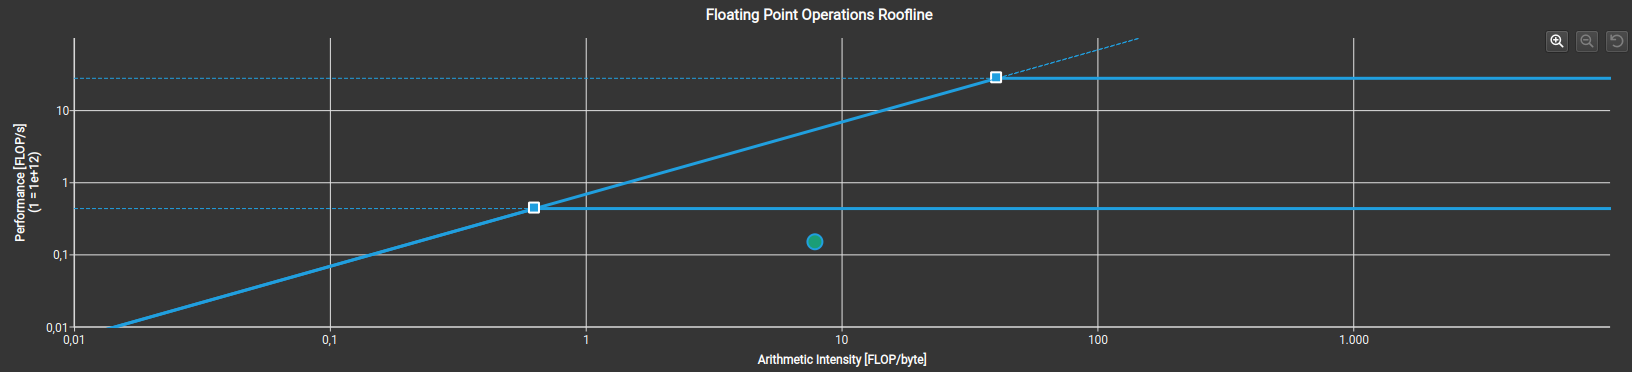
\includegraphics[width=\linewidth]{../resources/profiling/ncu/a40_after_DP_gpu32_p1M_neigh_roofline.png}
    \vspace{1\baselineskip}
    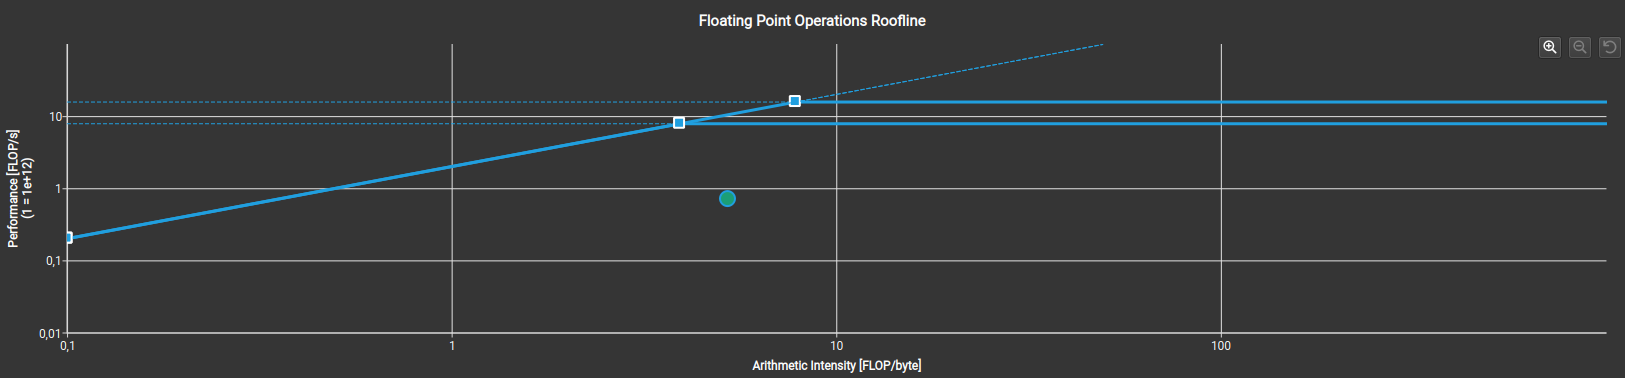
\includegraphics[width=\linewidth]{../resources/profiling/ncu/a100_after_DP_gpu256_p1M_neigh_roofline.png}
\end{frame}

\begin{frame}{Force computation performance roofline}
    \begin{tabular}{ c c c c }
        GPU  & Arith. Intensity 	& Througput   & Memory Throughput \\
        A40  & ~4.95 FLOP/byte		& 211 GFLOP/s & 40 GB/s\\
        A100 & 5.1 - 5.5 FLOP/byte	& 2.2 TFLOP/s & 410 GB/s
    \end{tabular}
    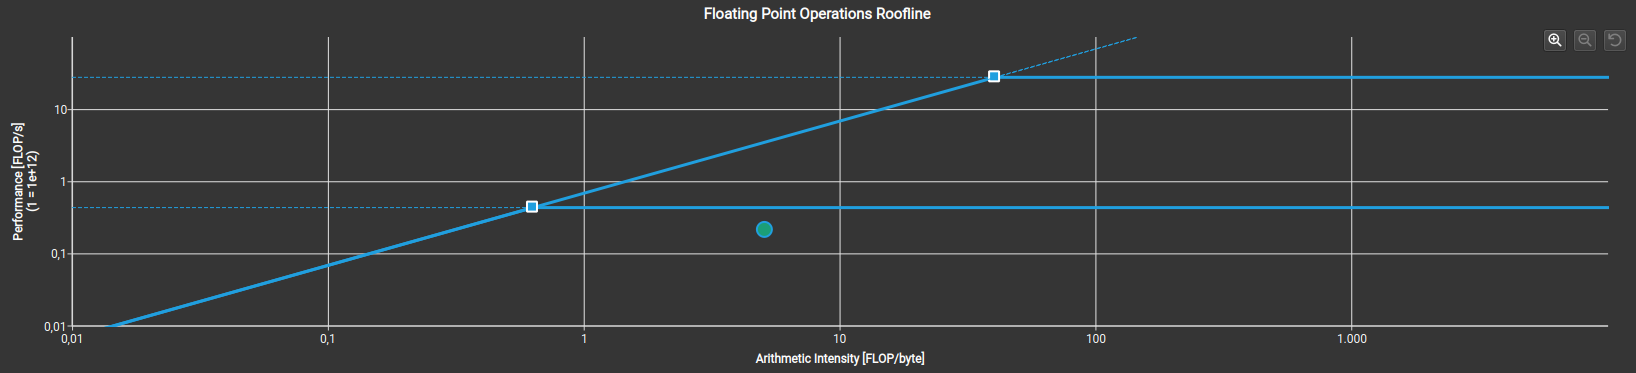
\includegraphics[width=\linewidth]{../resources/profiling/ncu/a40_after_DP_gpu32_p1M_force_roofline.png}
    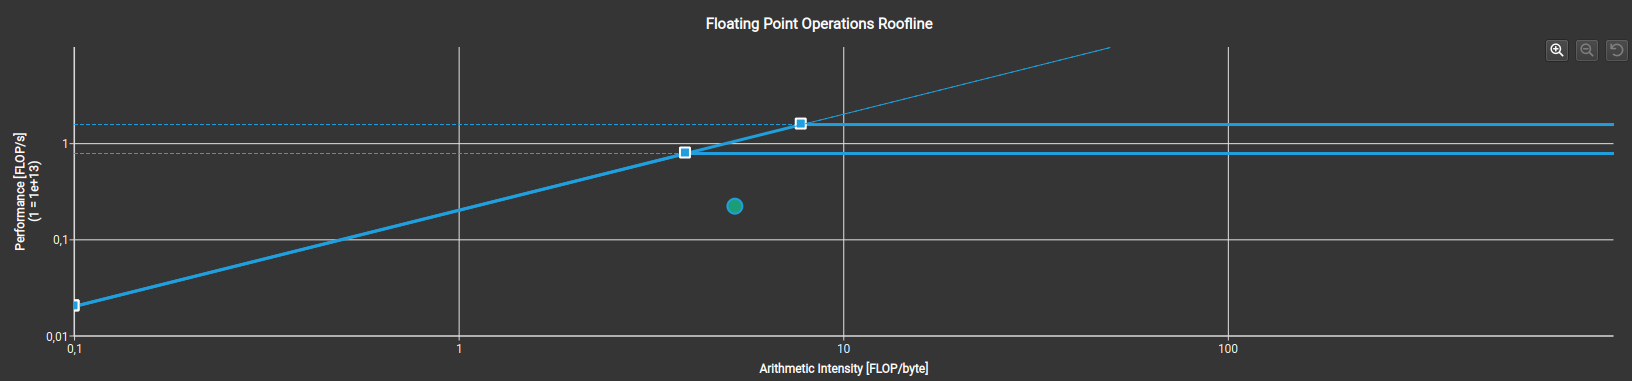
\includegraphics[width=\linewidth]{../resources/profiling/ncu/a100_after_DP_gpu256_p1M_force_roofline.png}
\end{frame}

\begin{frame}[fragile]{Project Description}{Simulation Process}
   
    \begin{small}
        \begin{Shaded}
            \begin{Highlighting}[]
                \ControlFlowTok{for}\NormalTok{ t }\KeywordTok{in}\NormalTok{ timesteps:}
                \ControlFlowTok{for}\NormalTok{ atom }\KeywordTok{in}\NormalTok{ atoms:}
                \NormalTok{    velocity[atom] }\OperatorTok{+=}\NormalTok{ force[atom]}
                \NormalTok{    position[atom] }\OperatorTok{+=}\NormalTok{ velocity[atom]}
                \ControlFlowTok{if}\NormalTok{ t }\OperatorTok{%} \DecValTok{20} \OperatorTok{==} \DecValTok{0}\NormalTok{:}
                    \NormalTok{neighbors }\OperatorTok{=}\NormalTok{ calculateNeighbors()}
                \ControlFlowTok{else:}
\color{red}                    \NormalTok{computeUpdatePbc()}
                \ControlFlowTok{for}\NormalTok{ atom }\KeywordTok{in}\NormalTok{ atoms:}
                \NormalTok{    neighbors }\OperatorTok{=}\NormalTok{ neighbors[atom]}
                \NormalTok{    force }\OperatorTok{=} \FloatTok{0.0}
                    \ControlFlowTok{for}\NormalTok{ neighbor }\KeywordTok{in}\NormalTok{ neighbors:}
                \NormalTok{        radius }\OperatorTok{=}\NormalTok{ calc_radius(...)}
                        \ControlFlowTok{if}\NormalTok{ radius }\OperatorTok{<}\NormalTok{ close_enough:}
                    \NormalTok{        force }\OperatorTok{+=}\NormalTok{ calc_force(...)}
                \NormalTok{    forces[atom] }\OperatorTok{+=}\NormalTok{ force}
                \end{Highlighting}
            \end{Shaded}
        \end{small}
    \end{frame}


\end{document}
